%%%--- Template for bachelor thesis at SfS, based on template
%%%--- for Diploma and Master thesis------
%%%------
\documentclass[11pt,a4paper,twoside,openright]{report}
\usepackage[english]{ETHDAsfs}%--> ETHDASA + fancyhdr + ... "umlaute"
%  + sfs-hyper -> hyperref 

\usepackage{pdfpages}%%to include the confirmation of originality (plagiarism
\usepackage{amsbsy}%% for \boldsymbol and \pmb{.}
\usepackage{amssymb}%% calls  amsfonts...
\usepackage{graphicx}%-- für PostScript-Grafiken (besser als  psfig!)
%\usepackage[draft]{graphicx} % grafics shown as boxes --> faster compilation
%
\usepackage[longnamesfirst]{natbib}%was {sfsbib}%- Für  Literatur-Referenzen
%           ^^^^^^^^^^^^^^ 1) "Hampel, Ronchetti, ..,"  2) "Hampel et al"
% Engineers (and other funny people) want to see [1], [2] 
% ---> use 'numbers' : \usepackage[longnamesfirst,number]{natbib}
%
%
\usepackage{texab}%- 'tex Abkürzungen' /u/sfs/tex/tex/latex/texab.sty
        %%- z.B.  \R, \Z, \Q, \Nat für reelle, ganze, rationale, natürl. Zahlen;
        %%-       \N   (Normalvert.)  \W == Wahrscheinlichkeit .....
        %%-  \med, \var, \Cov, \....
        %%-  \abs{x} == |x|   und   \norm{y} ==  || y ||   (aber anständig)
%% NOTE: texab contains many useful definitions and "shortcuts". It is
%% worth to open the file and have a look at them. HOWEVER, some
%% definitions are a bit can lead to conflicts with other packages. You
%% might for example want to comment out the line defininf \IF as an
%% operator when working with the algorithmic package, or to comment out
%% the line defining a command \Cite with working with the Biblatex package  
\usepackage{amsmath}
%\usepackage{mathrsfs}% Raph Smith's Formal Script font --> provides \mathscr
\usepackage[utf8]{inputenc}% <<------- Unicode, *NOT* iso-latin1 !
\usepackage{ae}% A[lmost] E[uropean] Fonts
\usepackage{enumerate}% Fuer selbstdefinierte Nummerierungen
%--------
\usepackage{relsize}%-> \smaller (etc) used here
\usepackage{color} %% to allow coloring in code listings
\usepackage{listings}% Fuer R-code, C-code, ....  and settings for these:
\definecolor{Mygrey}{gray}{0.75}% for linenumbers only!
\definecolor{Cgrey}{gray}{0.4}% for comments
\lstloadlanguages{R}
%%--- first version of "listings of R"-style : ---------------------------
% %% using \smaller here: makes R code listings use a *small* font:
% \lstset{language=R,basicstyle=\smaller[2],commentstyle=\rmfamily\smaller,
%   showstringspaces=false,xleftmargin=4ex,
%   literate={<-}{{$\leftarrow$}}1 {~}{{$\sim$}}1}
% \lstset{escapeinside={(*}{*)}} % for (*\ref{ }*) inside lstlistings (Scode) 
%\newcommand{\lil}[1]{\lstinline|#1|}
%%--- newer version of "listings of R"-style : ---------------------------
\lstset{%% Help, e.g. --> https://en.wikibooks.org/wiki/LaTeX/Source_Code_Listings
language=R,
basicstyle=\ttfamily\scriptsize,%%- \small > \footnotesize > \scriptsize > \tiny
%commentstyle=\ttfamily\color{Cgrey},
commentstyle=\itshape\color{Cgrey},
numbers=left,
numberstyle=\ttfamily\color{Mygrey}\tiny,
stepnumber=1,
numbersep=5pt,
backgroundcolor=\color{white},
showspaces=false,
showstringspaces=false,
showtabs=false,
frame=single,
tabsize=2,
captionpos=b,
breaklines=true,
%breakatwhitespace=false,
keywordstyle={},
morekeywords={},
xleftmargin=4ex, 
literate={<-}{{$\leftarrow$}}1 {~}{{$\sim$}}1}
\lstset{escapeinside={(*}{*)}} % for (*\ref{ }*) inside lstlistings (Scode) 
%%----------------------------------------------------------------------------

%%------- Theoreme ---
\newtheorem{definition}{Definition}[subsection]
\newtheorem{lemma}[definition]{Lemma}
\newtheorem{theorem}[definition]{Theorem}
\newtheorem{Coro}[definition]{Corollary}
\theoremstyle{definition} 
\newtheorem{example}[definition]{Example}
\newtheorem*{note}{Note}
\newtheorem*{remark}{Remark}

\DeclareMathOperator*{\plim}{plim}
\def\MR#1{\href{http://www.ams.org/mathscinet-getitem?mr=#1}{MR#1}}

\newcommand{\Lecture}[3]{\marginpar{#3.#2.#1}}
\newcommand{\Fu}{\mathcal{F}}
\newcommand{\aatop}[2]{\genfrac{}{}{0pt}{}{#1}{#2}}

%\renewcommand{\theequation}{\arabic{equation}}
\numberwithin{equation}{subsection}
%\includeonly{}

%\pscompress %--compress the Epsf .ps files and produce .bb -- WHEN dvips is run
%\psdraft%--- for quick pre-viewing (only shows frames)

%%%%%%%%%%%%%%%%%%%%%%%%%%%%%%%%%%%%%%%%%%%%%%%%%
%%% Path for your figures                      %%%
%%%%%%%%%%%%%%%%%%%%%%%%%%%%%%%%%%%%%%%%%%%%%%%%%
% Set the paths where all figures are taken from:
% \graphicspath{{/u/mueller/MA/Figures1/}{/u/mueller/MA/Figures2/}}

%%%%%%%%%%%%%%%%%%%%%%%%%%%%%%%%%%%%%%%%%%%%%%%%%
%%% Define your own commands here             %%%
%%%%%%%%%%%%%%%%%%%%%%%%%%%%%%%%%%%%%%%%%%%%%%%%%
\newcommand{\Bruch}[2]{{}^{#1}\!\!/\!_{#2}}
\renewcommand{\labelenumi}{\roman{enumi}.)}





\begin{document}
\bibliographystyle{chicago}% ---> Hampel,F., E.Ronchetti,... W.Stahel(1986) ...
 %was \bibliographystyle{sfsbib}\citationstyle{dcu} %OR DEFAULT : \citationstyle{agsm}

\pagenumbering{roman}%- roman numbering for first few pages

%%%%%%%%%%%%%%%%%%%%%%%%%%%%%%%%%%%%%%%%%%%%%%%%%
%%% Title page                                %%%
%%%%%%%%%%%%%%%%%%%%%%%%%%%%%%%%%%%%%%%%%%%%%%%%%
 \period{placeholder} %e.g. Winter 2019
 \dasatype{Bachelor Thesis}
 \students{placeholder} %e.g. Patrick M\"uller
 \mainreaderprefix{Adviser:}
 \mainreader{placeholder} %e.g. Prof. Dr. Martin M\"achler
 \alternatereaderprefix{}
 \alternatereader{}
 \issuedate{placeholder} %e.g. September 15th 2019
 \submissiondate{placeholder} %e.g. February 31st 2019
 \title{placeholder} %title of your work

 \maketitle%- Titelseite wird abgeschlossen
 %%~~~~~~~~~~~~~~~~~~~~~~~~~~~~~~~~~~~~~~~~

%%%%%%%%%%%%%%%%%%%%%%%%%%%%%%%%%%%%%%%%%%%%%%%%%
%%% Insert here acknowledgements and abstract %%%
%%%%%%%%%%%%%%%%%%%%%%%%%%%%%%%%%%%%%%%%%%%%%%%%%
 \newpage
\begin{abstract}
	The intent of this work is to compare The EM algorithm to a MLE approach in the
	case of multivariate normal mixture models using the Cholesky decomposition.
	The EM algorithm is widely used in statistics and is proven to converge, 
	however in pathological cases convergence slows down considerably. 
	MLE doesn't have this particular error, but is computationally costly.
	The Cholesky decomposition cuts down the necessary parameters almost in half....

	methods(not done)

	results(not done)% insert your abstract
\end{abstract}

%%%%%%%%%%%%%%%%%%%%%%%%%%%%%%%%%%%%%%%%%%%%%%%%%
%%% Table of contents and list of figures and %%%   
%%% tables (no need to change this usually)   %%%
%%%%%%%%%%%%%%%%%%%%%%%%%%%%%%%%%%%%%%%%%%%%%%%%%
\newpage
\tableofcontents
\newpage
\listoffigures
\newpage
\listoftables
\cleardoublepage

\pagenumbering{arabic}%--- switch back to standard numbering 


%%%%%%%%%%%%%%%%%%%%%%%%%%%%%%%%%%%%%%%%%%%%%%%%%
%%% Your text... Either write here directly,  %%%
%%% or even better: write in separate files   %%%
%%% that you just have to include here.       %%% 
%%%%%%%%%%%%%%%%%%%%%%%%%%%%%%%%%%%%%%%%%%%%%%%%%
\chapter{Introduction to normal mixture models}% Umlaute work thanks to \inputencoding{..} % in main file

\section{Definitions}

here intro to normal mixtures

A good and thorough introductory book is the work of McLachlan and Peel 2000 and
the reader is encouraged to study that to learn in depth about normal mixtures. 
We will here give a short overwiev of normal mixtures to fix notation and nomenclature.

Let $ \mu \in \mathbb{R}^p , \quad \Sigma \in \mathbb{R}^{p \times p} $ and 
$ \phi(\mu, \Sigma) $ be the normal distribution with
mean $ \mu $ and covariance matrix $ \Sigma $.

Normal mixture model are designed for situations where we assume that a given 
dataset originates from more than one population of explaining variables.

$ \pmb{Y}_1, \dots , \pmb{Y}_n $

\begin{definition}
    Suppose we have a random sample $ \pmb{Y}_1, \dots , \pmb{Y}_n $ with 
    probability density function $ \pmb{Y}_j \sim f(y_j) $ on $\mathbb{R}^p$
    We assume that the density $ f(y_j) $ of $ \pmb{Y}_j $ can be written in
    the form 

    \[ f(y_j) = \sum_{i=1}^{K} \pi_i \phi_i (y_i) \]

    The $ \pi_i $ are called the component densities of the mixture.
\end{definition}

explain in scetch EM algo

EM has desirable qualities like proven convergence, (give reference to dempster 1977 paper)

explain idea to use parameter optimizer instead,
EM has pathological insufficiencies, like 'getting stuck' for many iterations.
we hope we need less iterations, and as concequence less time.
'special' idea: using cholesky decomp.


\section{choice of notation}

describe difference in notation between ceuleux \& govaert and our covariance matrix decomposition.

The classification of models in this paper relies heavily on the work of Celeux and Grovaert,
however, out of necessity for clarity, we break with their notation. 
So as to not confuse the reader we describe here in depth the differences in notation
between Celeux and Govaert and ours.

explanation for the volume, shape and orientation descriptors

The basis of classification in CnG is the decomposition of a symmetric matrix into
an orthogonal and a diagonal component.
A symmetric positive definite matrix $ \Sigma $ can be decomposed as follows
\[ \Sigma = \lambda \pmb{D} \pmb{A} \pmb{D}^{\top} \]
with $ \pmb{D} $ an orthogonal matrix and $ \pmb{A} $ a diagonal matrix and 
$ \lambda = \sqrt[\uproot{3}p]{det(\Sigma)} $ the $ p-th $ root of the determinant 
of $ \Sigma $.

This decomposition has an appealing geometric interpretation, with $ \pmb{D} $ 
as the \textit{orientation} of the distribution, $ \pmb{A} $ the \textit{shape}, and $ \lambda $
the \textit{volume}.
The problem of notation comes from standard conventions in linear algebra, where
the letters $A$ and $D$ are usually occupied by arbytrary and diagonal matrices 
respectively. Furthermore, we intend to apply a variant of the Cholesky decomposition
to $ \Sigma $, the $ \pmb{L}\pmb{D}\pmb{L}^{\top} $ decomposition.
This obviously raises some conflicts in notation.

Therefore we, from here on, when reffering to the decomposition as described
by cng, will use the following modification of notation:

\begin{align*} 
    \pmb{D} \longmapsto \pmb{Q} \\
    \pmb{A} \longmapsto \pmb{\Lambda} \\
    \lambda \longmapsto \alpha  \\
    \Sigma = \lambda \pmb{D} \pmb{A} \pmb{D}^{\top} =
        \alpha \pmb{Q} \pmb{\Lambda} \pmb{Q}^{\top}
\end{align*}

These were chosen according to general conventions of linear algebra.
$ \pmb{Q} $ is usually chosen for orthonormal matrices; $ \pmb{\Lambda} $ is 
often a choice for eigen vectors and $ \alpha $ was somewhat arbitrarily chosen.


make clear that the models can not be translated one to one to ldlt model

make nice table(maybe sideways to account for parameter list)


\begin{table}[!htb]
    \centering
\rotatebox{90}
{
    \begin{tabular}{| c | c c c c c c | c c c |}
        \hline
        Model & $\pmb{\Sigma}_k$ C\&G & volume & shape & orientation & parameters & count & $ \pmb{LDL}^\top $ & parameters & count \\
        \hline

        EII    & $ \alpha \pmb{I} $ & equal & equal & - & $ \alpha $ & 1 & same as C\&G & & \\
        VII    & $ \alpha_k \pmb{I} $         & variable & equal & - & $ \alpha_k $ & $ K $ & & & \\
        EEI    & $ \alpha \pmb{\Lambda} $     & equal & equal & coordinate axes & $ \alpha, \lambda_i $ & $ 1+p $ & & & \\
        VEI    & $ \alpha_k \pmb{\Lambda} $ & variable & equal & coordinate axes & $ \alpha_k, \lambda_{i}$ & $ K+p $ & & & \\
        EVI    & $ \alpha \pmb{\Lambda}_k $ &equal & variable & coordinate axes & $ \alpha, \lambda_{i,k} $ & $ 1+pK $ & & & \\
        VVI    & $ \alpha_k \pmb{\Lambda}_k $ & variable & variable & coordinate axes & $ \alpha_k, \lambda_{i,k} $ & $ K+pK $ & & & \\
        \hline
        EEE    & $ \alpha \pmb{Q \Lambda Q}^\top $ &equal & equal & equal & $ \alpha, \lambda_{i}, q_{i,j} $ & $ 1+p+p^2 $ & $ \alpha \pmb{LDL}^{\top} $ & & \\
        \hline
        EVE    & $ \alpha \pmb{Q \Lambda}_k \pmb{Q}^\top $ &equal & variable & equal & $ \alpha, \lambda_{i,k}, q_{i,j} $ & $ 1+pK+p^2 $ & doesn't exist & & \\
        \hline
        VEE    & $ \alpha_k \pmb{Q \Lambda Q}^\top $ & variable & equal & equal & $ \alpha_k, \lambda_{i}, q_{i,j} $ & $ K+p+p^2 $ & $ \alpha_k \pmb{LDL}^\top $ & & \\
        \hline
        VVE    & $ \alpha_k \pmb{Q \Lambda}_k \pmb{Q}^\top $ &variable & variable & equal & $ \alpha_k, \lambda_{i,k}, q_{i,j} $ & $ K+pK+p^2 $ & & & \\
        EEV    & $ \alpha \pmb{Q}_k \pmb{\Lambda} \pmb{Q}_k^\top $ &equal & equal & variable & $ \alpha, \lambda_{i}, q_{i,j,k} $ & $ 1+p+Kp^2 $ &    & & \\
        VEV    & $ \alpha_k \pmb{Q}_k \pmb{\Lambda} \pmb{Q}_k^\top $ &variable & equal & variable & $ \alpha_k, \lambda_{i}, q_{i,j,k} $ & $ K+p+Kp^2 $ & & & \\
        \hline
        EVV    & $ \alpha \pmb{Q}_k \pmb{\Lambda}_k \pmb{Q}_k^\top $ & equal & variable & variable & $ \alpha, \lambda_{i}, q_{i,j,k} $ & $ 1+pK+Kp^2 $ & $ \alpha \pmb{L}_k \pmb{D}_k \pmb{L}_k^\top $ & $ \lambda, d_{i,k}, l_{i,j,k}\ j>i $ & $ 1+pK+K\frac{p(p-1)}{2} $ \\
        VVV    & $ \alpha_k \pmb{Q}_k \pmb{\Lambda}_k \pmb{Q}_k^\top $ & variable & variable & variable & $ \alpha_k, \lambda_{i}, q_{i,j,k} $ & $ K+pK+Kp^2 $ & $ \alpha_k \pmb{L}_k \pmb{D}_k \pmb{L}_k^\top $ & $ \lambda_k, d_{i,k}, l_{i,j,k}\ j>i $ & $ K+pK+K\frac{p(p-1)}{2} $ \\
        \hline
    \end{tabular}

    \label{table:1}

}

\caption{Table of Parameters}

\end{table}


\clearpage

\section{problems of EM}


the EM algo has stalling problems especially close to a local optimum

show an example using nor1mix


\begin{Schunk}
\begin{Sinput}
> library("nor1mix")
> plot(MW.nm9, lty=2, col = "blue", p.norm=FALSE, p.comp=TRUE)
> set.seed(2019)
> x9 <- rnorMix(5000, MW.nm9)
> lines(density(x9), lwd=1.8)# "clearly" 3 components
\end{Sinput}
\end{Schunk}
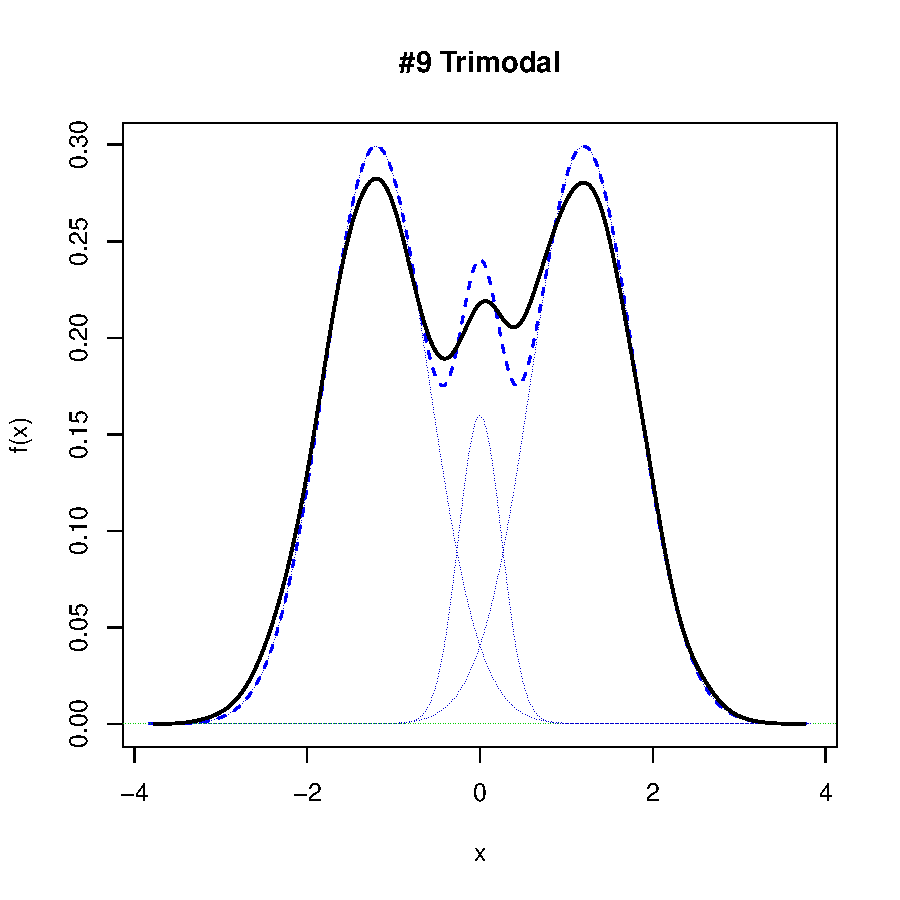
\includegraphics{chapter1-001}


then an illustration of MW examples of pathological cases


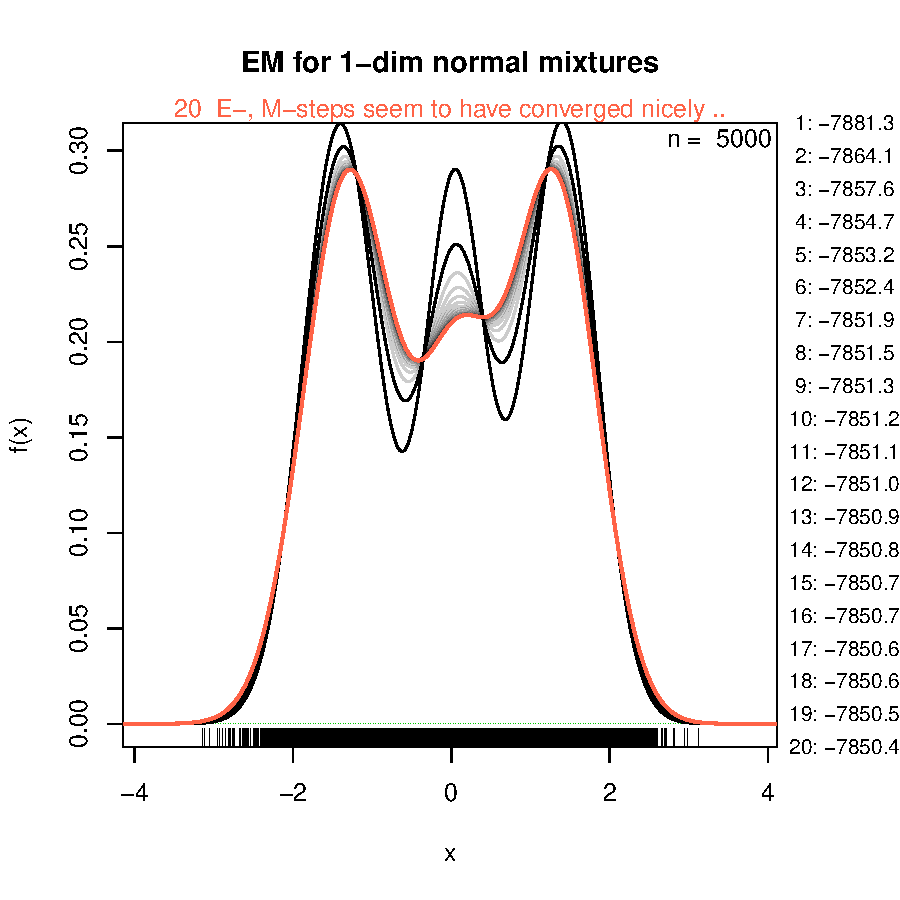
\includegraphics{chapter1-002}


yay, got figure to print. solution was use of fig=TRUE, instead of various mutations like figure=true.

here we see how change in loglik seems to stagnate. However, this does not stay that way, if we let EM run a bit further.

\begin{Schunk}
\begin{Sinput}
> r <- p.EMsteps(200, x9, nm1)
\end{Sinput}
\end{Schunk}
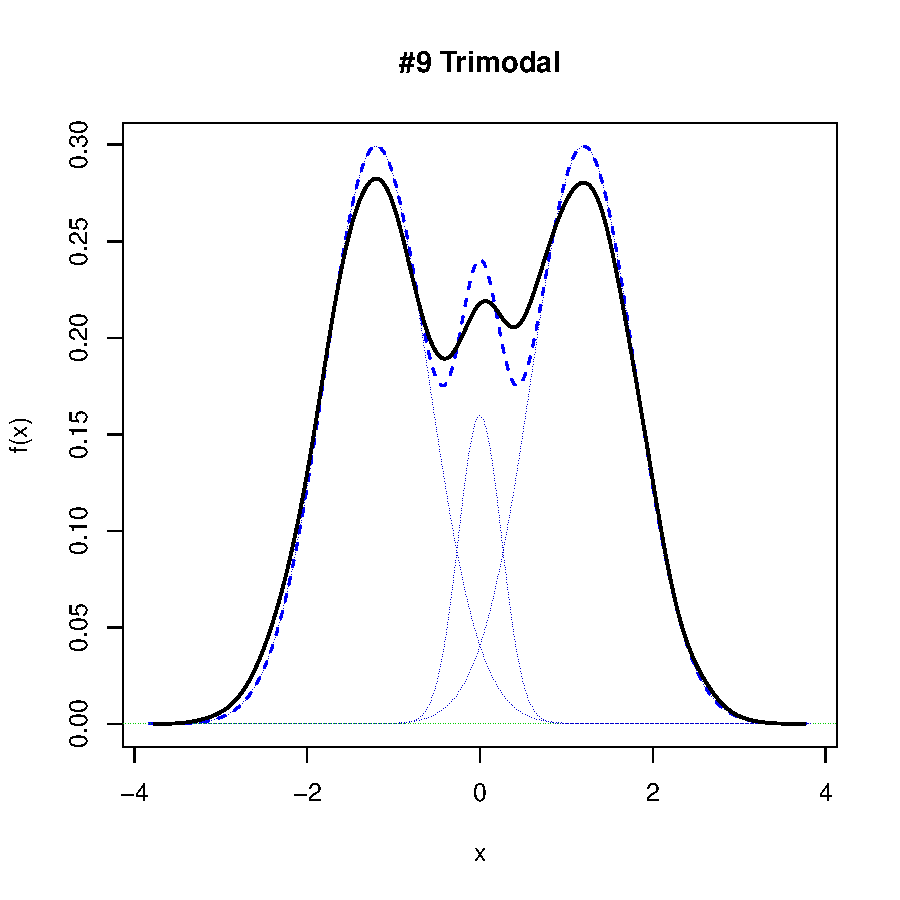
\includegraphics{chapter1-003}

to conclude example show part of mixest that shows it takes 1200 iterations to converge

In fact, it seems that the previous solution is a saddle point in the likelihood function, where EM has chronic problems continuing improvements.

should include animations?? like mix\_est\_1d.R line 249+24 lines

maybe show Marr Wand's examples of 'difficult' mixtures

give conclusion recapping the just demonstrated, and lead in for next chapter






\chapter{The {\tt norMmix} Package}

explain, that this package was written purposefully for this paper.

The norMmix package is constructed around the {\tt norMmix} object, that codifies a {\tt nor}mal {\tt M}ultivariate {\tt mix}ture model,  and the {\tt llnorMmix()} function.

quickly list contents of norMmix object

relies on {\tt optim()} generic optimizer. maximizes llnormix by varying model parameters.

since mclust is one of the more popular packages implementing the EM algo, we employ a lot of functions from mclust, to keep things around EM as similar as possible.

\section{concept of package} (this Section maybe one chapter earlier)

about Cholesky decomp as ldlt. has advantages: fast, parametrically parsimonious, can easily compute loglikelihood

maybe reread section in McLachlan about accelerating EM algo

not possible to sensibly compare normal mixtures except maybe a strange sorting algorithm using mahalanobis distance or Kullback-Leibler distance or similar(Hellinger), but not numerically sensible to integrate over potentially high-dimensional spaces.

So caomparison of algos done through throwing difficult mixtures and non-mixtures at it and hoping that norMmix finds better solutions than EM. So the criteria for "better fit" are 1. better log-likelihood 2. correct model, where EM fails.

\section{finer details of {\tt norMmix} package}




\chapter{Comparing Algotithms}

display abilities of norMmix on its own. can find correct models

maybe apply to MW[0-9] objects?

not sure


\chapter{Coclusions}

\chapter{The {\tt norMmix} Package}





\section{Introduction to the Package}

% it 1
For this thesis, an \Rp package was developed that implements the algorithm
that fits multivariate normal mixtures to given data.
\footnote{The package was written with \Rp version 3.6.1 (2019-07-05) last 
updated on 2019-10-22.}
There is a lot of unused code still in the package. These were at one point
implemented used and discarded. They are still included for demonstration.
The {\tt norMmix} package is constructed around the {\tt norMmix} object, that 
codifies a {\tt nor}mal {\tt M}ultivariate {\tt mix}ture model,  and the {\tt 
llnorMmix()} function, that calculates the log-likelihood given a model and 
data.


%% table of params
%% TODO: description of table
\begin{table}
    \centering
    \begin{tabular}{l l}
        \hline
        In Notation & In Code \\
        \hline
        $\pi_i$     & {\tt w, weights} \\
        $\Sigma$    & {\tt Sigma} \\
        $\mu$       & {\tt mu} \\
        $K$         & {\tt k} \\
        dimension   & {\tt p, dim, dims} \\
        components  & {\tt cl, components} \\
        \hline
    \end{tabular}
    \caption{Translation Table: Mathematical Notation to \Rp Code}
    \label{tab:code-notation}
\end{table}


% it 1
The package contains the following functionality:
\begin{table}
\begin{description}
    \item [norMmix] {\tt norMmix()} is the 'init-method' for 
        {\tt norMmix} objects. There exist {\tt is.norMmix} {\tt rnorMmix} and
        {\tt dnorMmix} functions.
    \item [parametrization] The main functions that handle reparametrization
        of models from and to $\pmb{LDL}^\top$ decomposition are {\tt nMm2par}
        and {\tt par2nMm}, which are inverse to each other.
    \item [MLE] The function {\tt norMmixMLE} marries the main components of 
        this package. It initializes a model and parametrizes it for use with 
        {\tt optim}
    \item [model choice] Using {\tt norMmixMLE}, the function fitnMm allows fitting 
        of multiple models and components. Functions analyzing the output of 
        this are also provided, e.g. {\tt BIC} and {\tt print} methods.
    \item [misc] There are also various methods of generics, like {\tt logLik,
        print, BIC, AIC} and {\tt nobs} as well as various {\tt print} methods.
    \item [example objects] Following the paper of \cite{Mar92} various example
        objects are provided and used for study. They follow the naming 
        convention: MW + dimension + number. for example {\tt MW213} for the 
        13-th model of dimension 2.
    \item [simulations] The purpose of this package is to study simulations. 
        there are functions provided to study large collections of evaluated 
        data. e.g {\tt epfl} %TODO: describe and give ref.
\end{description}
\end{table}

relies on {\tt optim()} generic optimizer. maximizes llnormix by varying model 
parameters.

since mclust is one of the more popular packages implementing the EM algo, we 
employ a lot of functions from mclust, to keep things around EM as similar as 
possible.

% it 1
Conceptually, at the start of a fitting algo, e.g. EM we need to initialize a
mixture object. % TODO we (will?) have translation methods to and from mclust
thereafter the paths diverge. at the heart of norMmix's functionality
lie the functions: llnorMmix and nMm2par which are in turn employed by 
norMmixMLE to funnel a mixture object into optim and give optim a function
to optimize.

also relies on {\tt mixtools} package for random generating function 
{\tt rnorMmix} using {\tt rmvnorm}.

\section{On The Development of {\tt norMmix}}

about Cholesky decomp as ldlt. has advantages: fast, parametrically 
parsimonious, can easily compute loglikelihood

%it 1

maybe reread section in McLachlan about accelerating EM algo

not possible to sensibly compare normal mixtures except maybe a strange sorting 
algorithm using Mahalanobis distance or Kullback-Leibler distance or similar
(Hellinger), but not numerically sensible to integrate over potentially 
high-dimensional spaces.

%% TODO: explain comparison


general list of (not necessarily mathematical) dead-ends in the development 
life of the norMmix package.
argue why this is in this section?? because, as a BScT, the learning is as much
part of the research as the results.


% it 1
One dead-end was the parametrization of the weights of a mixture using the 
{\tt logit} function.

\begin{Schunk}
\begin{Sinput}
> logit <- function(e) {
+     stopifnot(is.numeric(e) ,all(e >= 0), all.equal(sum(e),1))
+     qlogis(e[-1L])
+ }
> logitinv <- function(e) {
+     if (length(e)==0) {return(c(1))}
+     stopifnot(is.numeric(e))
+     e<- plogis(e)
+     sp. <- sum(e)
+     w <- c((1-sp.), e)
+ }
\end{Sinput}
\end{Schunk}

This uses the logistical function {\tt logis} to transform to reduce the number
of weights from $K$ to $K-1$. Much like {\tt clr1}, given a list of weights 
{\tt logit} will transform them and {\tt logitinv} will correctly reverse the 
transformation. However, unlike {\tt clr1}, it will not transform an arbitrary 
list of length $K-1$ into a valid weight parameter. For example:

\begin{Schunk}
\begin{Sinput}
> w <- runif(7); ret <- logitinv(w)
> ret
\end{Sinput}
\begin{Soutput}
[1] -3.2617309  0.6306458  0.5682759  0.5602498  0.6616009  0.6906020  0.5707690
[8]  0.5795875
\end{Soutput}
\end{Schunk}

The issue here is that the last line of {\tt logitinv}, which is necessary to 
sum to one, but results in a negative value in {\tt ret[1]} which is not a 
valid weight. The underlying issue is that not every tuple in $\R^{K-1}$ is 
a result of {\tt logit}.

The option to use {\tt logit} is still an argument to {\tt norMmixMLE} by 
specifying {\tt trafo="logit"}, but it shouldn't be used.


% it 1
Another issue during development cropped up during fitting of high dimensional
data. We studied the dataset {\tt SMI.12} from the package {\tt copula}:

\begin{Schunk}
\begin{Sinput}
> data(SMI.12, package="copula")
> str(SMI.12)
\end{Sinput}
\begin{Soutput}
 num [1:141, 1:20] 16.1 15.7 15.7 16.1 16.6 ...
 - attr(*, "dimnames")=List of 2
  ..$ : chr [1:141] "2011-09-09" "2011-09-12" "2011-09-13" "2011-09-14" ...
  ..$ : chr [1:20] "ABBN" "ATLN" "ADEN" "CSGN" ...
\end{Soutput}
\end{Schunk}

A consequence of high dimensions is that matrix multiplication is no longer
very stable. As a result, the covariance matrices produced by our own 
implementation of the EM-algorithms m-step ({\tt mstep.nMm}) were not positive
definite.
In the case of {\tt SMI.12}, several covariance matrices are degenerate, which
results in cancellation error with near-zero entries.
We attempted to correct this with the function {\tt forcePositive}, which 
simply tries to set $\pmb{D}$ in $\pmb{LDL}^\top$ greater than zero.
This didn't resolve the issue, since a non-negligible part of the numerical
error was in the $\pmb{L}$ matrix and the resultant covariance matrix was still
not positive definite.

We eventually resolved this issue by abandoning our own implementation and 
using the functions from the {\tt Mclust} package. Not only were these 
numerically stable they were also able to differentiate between models, whereas
ours would assume VVV for every fit.

testing of mvtnorm as proof that ldlt is in fact faster parametrization

mention, that there may be faster ways to apply backsolve. 
quote knuth about premature optimization?

\section{Demonstration}

Mention, that mclust doesn't depend on seed(double check) and therefore norMmix has 
'advantage' of 'confidence intervals'. We can run 50 simulations and see if there
might be more sensible clusters.


% it 1
demonstrate things; essentially put .Rd example sections here

%% and more
% \include{....}
 
%%%%%%%%%%%%%%%%%%%%%%%%%%%%%%%%%%%%%%%%%%%%%%%%%
%%% Bibliography                              %%%
%%%%%%%%%%%%%%%%%%%%%%%%%%%%%%%%%%%%%%%%%%%%%%%%%
\addtocontents{toc}{\vspace{.5\baselineskip}}
% \cleardoublepage
\phantomsection
\addcontentsline{toc}{chapter}{\protect\numberline{}{Bibliography}}
\bibliography{myReferences}
%% All books from our library (SfS) are already in a BiBTeX file
%% 'Assbib.bib' (included here as well), using
% \bibliography{myReferences,Assbib}
% ---------------------------------- instead of the above

%%%%%%%%%%%%%%%%%%%%%%%%%%%%%%%%%%%%%%%%%%%%%%%%% 
%%% Appendices (if needed, e.g. for R code)   %%%
%%%%%%%%%%%%%%%%%%%%%%%%%%%%%%%%%%%%%%%%%%%%%%%%%
\addtocontents{toc}{\vspace{.5\baselineskip}}
\appendix
% outcommented \chapter{Complementary information}
\label{app:complement}

Additional material. For example long mathematical derivations could be
given in the appendix. Or you could include part of your code that is
needed in printed form. You can add several Appendices to your thesis (as
you can include several chapters in the main part of your work).

\section{Including \Rp code with verbatim}
A simple (rather too simple, see~\ref{App:listings}) way to include code or
{\it R} output is to use 
\texttt{verbatim}. It just prints the text however it is (including all
spaces, ``strange'' symbols,...) in a slightly different font.
\begin{verbatim}
## loading packages
library(RBGL)
library(Rgraphviz)
library(boot)

## global variables
X_MAX <- 150

   This allows me to put as many s  p a   c es   as I want.
I can also use \ and ` and & and all the rest that is usually only 
accepted in the math mode.

I can also make as 
                  many 
             line 
    breaks as 
I want... and
             where I want. 
\end{verbatim}

But really recommended,  much better is the following:

\section{Including \Rp code with the \emph{listings} package}\label{App:listings}
However, it is much nicer to use the \emph{listings} package to include \Rp
code in your report. It allows you to number the lines, color the comments
differently than the code, and so on.
All the following is produced by simply writing

or \verb!\lstinputlisting{/u/maechler/R/Pkgs/sfsmisc/R/ellipse.R}! :

\lstinputlisting{ellipse.R}% was /u/maechler/R/Pkgs/sfsmisc/R/ellipse.R

\section{Using Sweave to include \Rp code (and more) in your report}
The easiest (and most elegant) way to include \Rp code and its output (and
have all your figures up to date with your report) is to use Sweave. You
can find an introduction Sweave in \texttt{/u/sfs/StatSoftDoc/Sweave/Sweave-tutorial.pdf}.

%%% Local Variables: 
%%% mode: latex
%%% TeX-master: "BachelorThesisSfS"
%%% End: 

% outcommented \chapter{2nd Appendix: More sophisticated R code listing} \label{appendix-more-R}

Chapter-wise listing of parts of R code, using
\begin{itemize}
\item \texttt{firstline=n1}
\item \texttt{lastline=n2}
\item \texttt{title=<text>}
\end{itemize}
e.g., for the first example below
\begin{verbatim}
\lstinputlisting[firstline=1,lastline=32,
                 title= \texttt{read\_irwls\_fn.R}]{../RCode/read_irwls_fn.R}
\end{verbatim}

% \section{Chapter 2} \label{app 2}

% \lstinputlisting[firstline=1,lastline=77,
% title=\texttt{analytic\_efficiency.R}]{../RCode/analytic_efficiency.R}
% %\lstinputlisting[firstline=,lastline=]{../RCode/???.R}

\bigskip% or even  \clearpage

%-----------------------------------------------------------------------------------------
\section{Chapter 5} \label{app 5}

% \lstinputlisting[firstline=1,lastline=71,
%                  title=\texttt{loss-fn\_rotated.R}]{../RCode/loss-fn_rotated.R}
%\lstinputlisting[firstline=1,lastline=32,
%                 title= \texttt{read\_irwls\_fn.R}]{../RCode/read_irwls_fn.R}

\medskip
                 
%\lstinputlisting[firstline=1,lastline=45,title=\texttt{plot.psi.R}]{../RCode/plot.psi.R}
%\lstinputlisting[firstline=,lastline=]{../RCode/???.R}
%\lstinputlisting[firstline=,lastline=]{../RCode/???.R}

% \clearpage
%-----------------------------------------------------------------------------------------
% \section{Chapter 7} \label{app 7}

% \lstinputlisting[firstline=1,lastline=35,
%                  title= \texttt{stat.test} from \texttt{lmrob2-fn.R}]{../RCode/lmrob2-fn.R}
% \lstinputlisting[firstline=41,lastline=194,
%                  title=\texttt{M.optimal.ms} from \texttt{lmrob2-fn.R}]{../RCode/lmrob2-fn.R}
%\lstinputlisting[firstline=,lastline=]{../RCode/???.R}
%-----------------------------------------------------------------------------------------

%%% Local Variables:
%%% mode: latex
%%% TeX-master: "MasterThesisSfS"
%%% End:


%%%%%%%%%%%%%%%%%%%%%%%%%%%%%%%%%%%%%%%%%%%%%%%%%% 
%%% Declaration of originality (Do not remove!)%%%
%%%%%%%%%%%%%%%%%%%%%%%%%%%%%%%%%%%%%%%%%%%%%%%%%%
%% Instructions:
%% -------------
%% fill in the empty document confirmation-originality.pdf electronically
%% print it out and sign it
%% scan it in again and save the scan in this directory with name
%% confirmation-originality-scan.pdf 
%%
%% General info on plagiarism:
%% https://www.ethz.ch/students/en/studies/performance-assessments/plagiarism.html 
\cleardoublepage
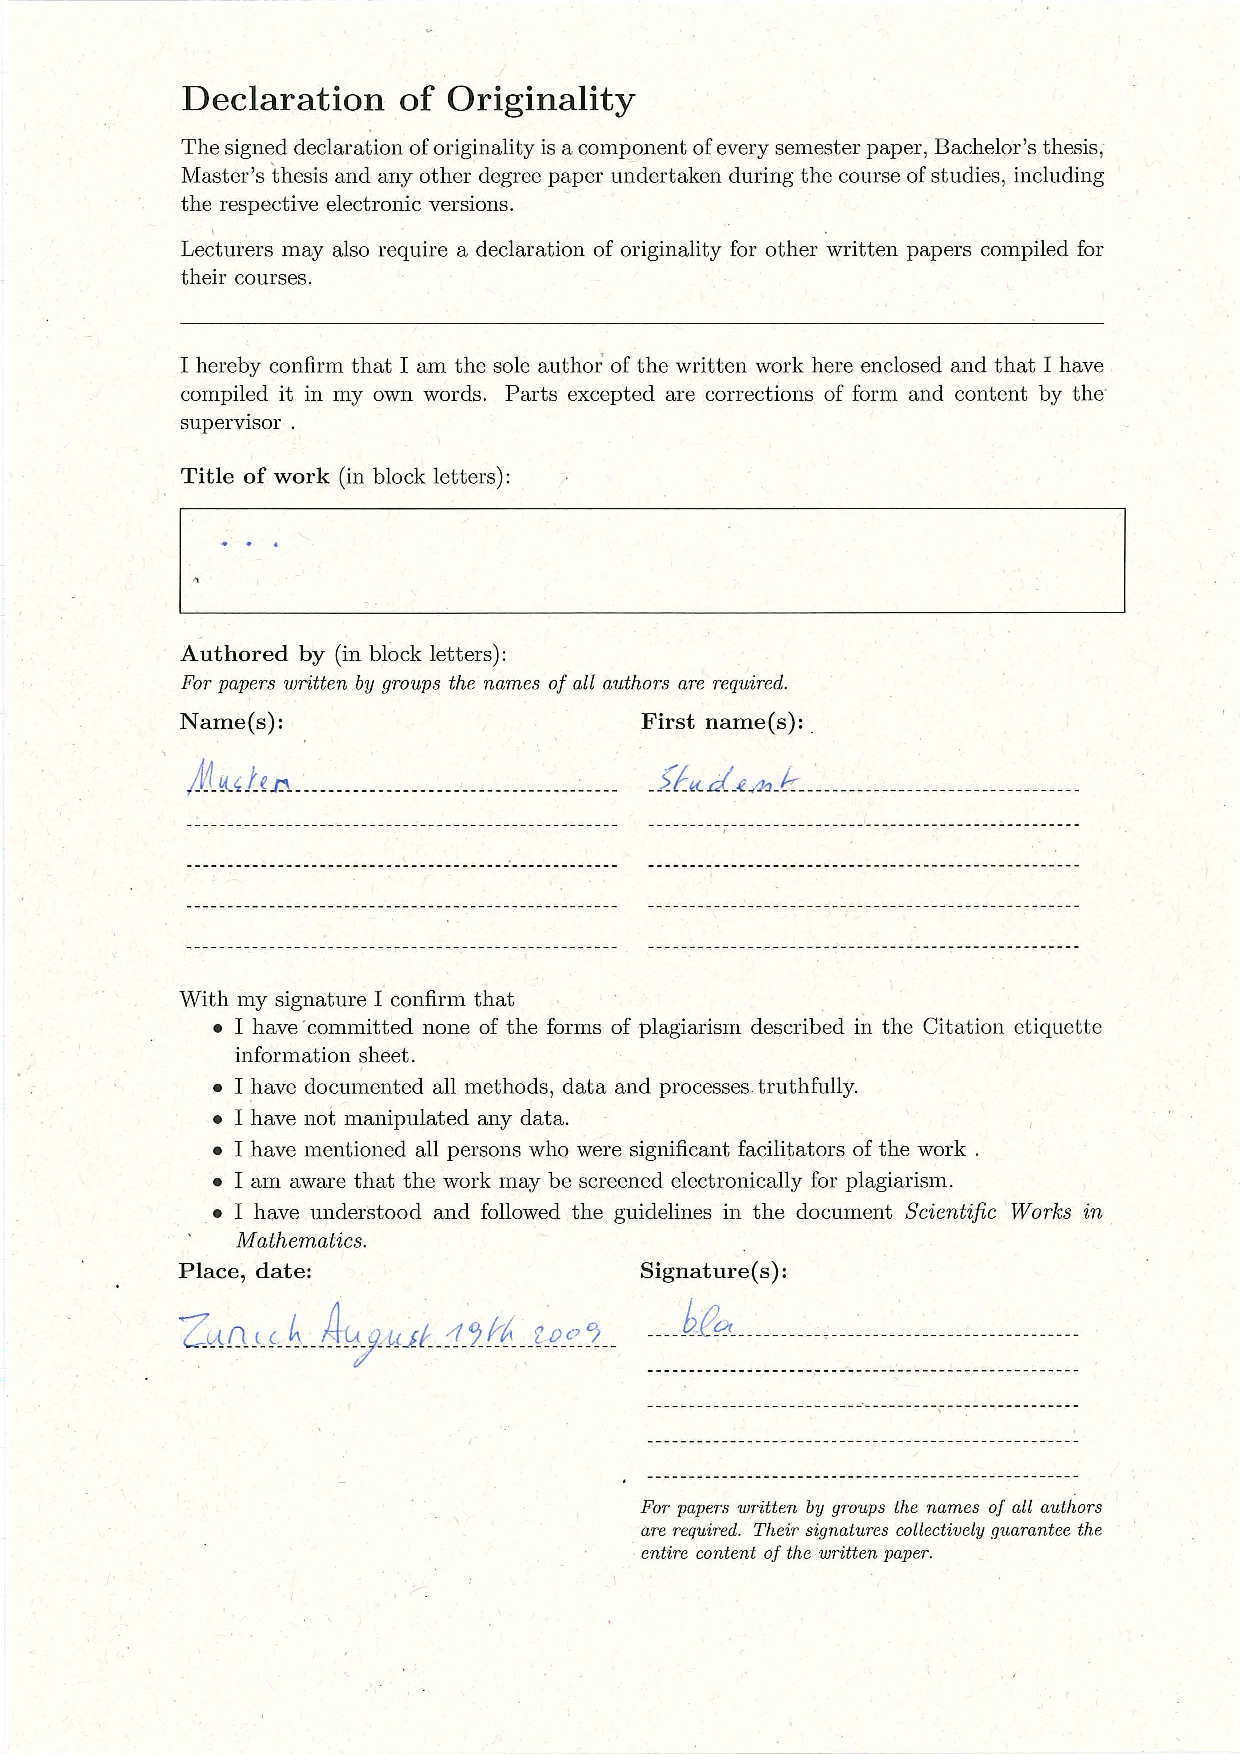
\includepdf[pages={-}, frame=true,scale=1]{confirmation-originality-scan.pdf}
\end{document}
